\documentclass[12pt]{scrreprt}
\usepackage{graphicx}


\graphicspath{{./img/}}

% Title Page
\title{Deliverable \#1}
\author{Team D\'evlopp}


\begin{document}
\maketitle
\tableofcontents

\section{The team}
We are team D\'evlopp. Our logo can be seen on the title page.

\subsection{Team photos}
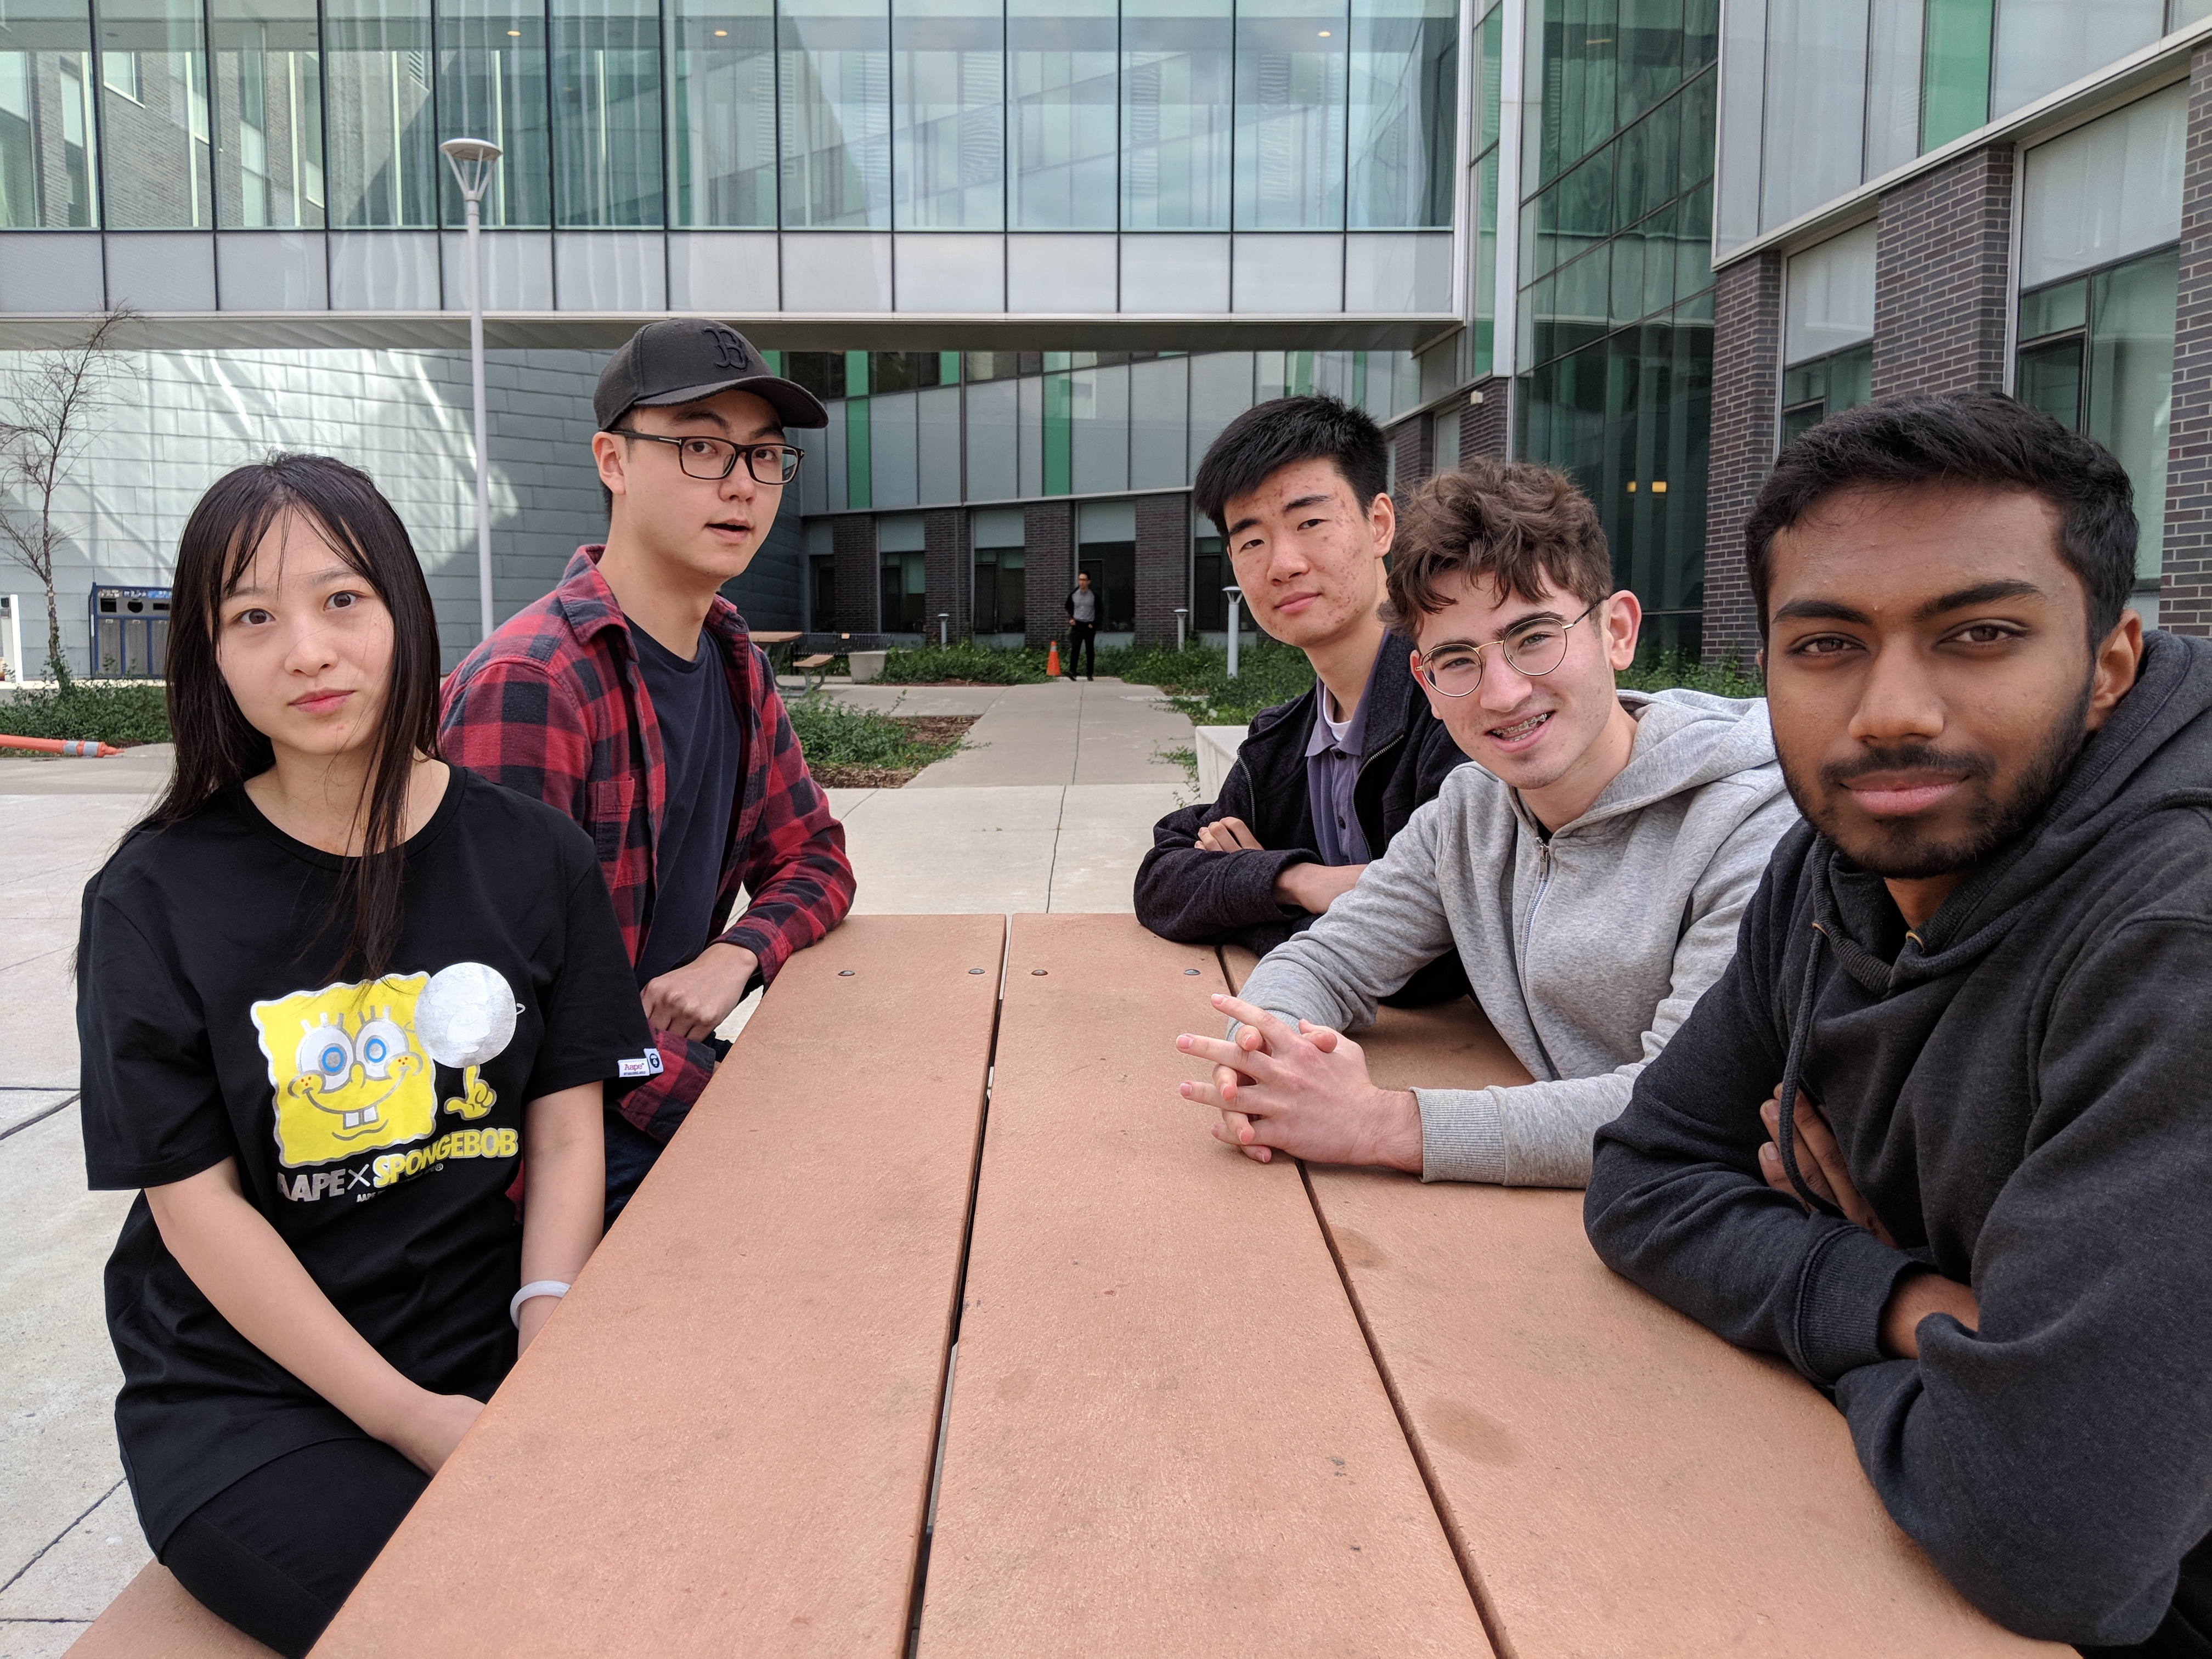
\includegraphics[width=0.9\textwidth]{team.jpg}


\subsection{Our goals}

\subsection{Our strengths}
Logic 2010 is an internet-assisted classroom instruction and assignment tool used in first-order logic courses at schools like UCLA and UofT. The tool consists of a desktop application, and a per-course web page. The web page allows students to view the assigned problems for the week, their completion state, course notes and other handouts. The problems are completed and submitted using the desktop application. The application is separated into modules for each of the sections covered in the course. The modules contain problems specific to the section they cover. Each module has a different way of inputting solutions to the problems, since the problem types vary. The desktop application checks each problem when it is completed, and indicates if it is correct. The student can then submit their work when they are satisfied with it.

\end{document}          
